\chapter{Method}

This chapter presents the data used for training and evaluating models, the models I will test and how the text is processed to be of appropriate format for the models. 

The financial indices I considered in this project are the S\&P 500 and the US treasury rate with 1 and 3 years to maturity:
\begin{itemize}
    \item S\&P 500 (\textit{Standard \& Poor's}) is a stock market index reflecting the performance of the 500 largest companies listed on the stock exchanges in the United States.
    \item The US Treasury rate with maturity $n$ is the yield on a government zero coupon bond with the same maturity. 
\end{itemize}


\section{Data Collection and Pre-Processing}

All models are trained on two datasets -- a labeled movie review dataset from IMDb for benchmarking and an unlabeled financial news dataset from Reuters combined with time series data for the financial interpretation. 

\subsection{IMDd Dataset -- Benchmarking}
The IMDb dataset is a commonly used benchmarking dataset for binary classification of text data. The dataset was compiled by \citet{maas-EtAl:2011:ACL-HLT2011} and contains 50,000 polarized movie reviews with 25,000 positive and negative reviews respectively. Evaluating models on this dataset can validate that the models can capture some meaningful information from text data and thus give better insight about the performance on the financial task. It also  generally confirms that the model is implemented appropriately. For comparison, \citeauthor{xie2019unsupervised} achieved 95.8\% accuracy using BERT large and unsupervised data augmentation on the IMDb dataset. This is in the state of the art-region, even though there are models that have scored slightly higher. 

Two reviews are presented below, first a positive one and then a negative one. 

\begin{quote}
    ``This program was quite interesting. The way the program was displayed made it all the more interesting. String Theory is also very interesting to listen too. The whole three hours in my opinion were well worth it. I enjoyed listening to the ideas given by the physicists. Extra dimensions really boggle the mind. If you have the chance, watch this amazing documentary'' 
\end{quote}
\begin{quote}
    ``There wasn't a 0 in the voting option so i was compelled to use the next available figure. It is a sad day for bollywood when such type of movies which have star-cast actors is nothing more are than a bunch of juvenile acting, and an awful script. This movie is nowhere near to be called a clone of Hitch. Salman khan with his usual take-off-you-shirt theme and Govinda with his in-humorous laughs. If somebody had told 2 decades ago that I would be writing a comment on Salman (after his success with Maine Pyar Kiya), I would have written him/her off. ''
\end{quote}

\subsection{Reuters Financial News Dataset}

The corpus used for this project consists of 109,110 financial news articles from Reuters. It was first compiled and used by \citet{ding2014using} for predicting stock price direction. Only the titles of the news data is used to train the model, as suggested by \citet{ding2014using}. The reasoning behind this is that including the contents of the articles do not significantly improve the model. 

The data contains financial news regarding the US market from the 10th of October 2006 to the 11th of November 2013, with approximately 5-50 news articles per day and is publicly available\footnote{Available at \url{https://github.com/duynht/financial-news-dataset}.}. A few examples of headlines follows. 

\begin{quote}
    2006-12-18 -- ``Shares fall on tech worries, oil stocks'' \\
    2008-09-12 -- ``S\&P analyst says does not expect Lehman to fail'' \\
    2008-09-15 -- ``Lehman files for bankruptcy, plans to sell units'' \\ 
    2010-06-22 -- ``Market ends down on housing data and technicals '' \\
    2012-04-11 -- ``U.S. weighs higher threshold for swap dealers: report'' \\
\end{quote}


\subsubsection{Pre-Processing}

The first part of the pre-processing of text data is similar for all models. The intersection of dates available with news data and financial data is assessed and headlines for these days are extracted. The text is quite clean since it is the headlines of published news articles. It does not require as much cleaning as for instance a corpus of tweets. 

The next step of the pre-processing is to tokenize the data. This is done differently depending on what model to use, but a parameter that is set for all models is the \textit{vocabulary size}. The vocabulary size is simply the amount of words to keep track of. Keras has a tokenization functionality which includes words based on frequency -- the most common words are included. How the tokenization is performed for each model is explained more carefully under each section.

For some of the used models the natural language processing part can be seen as pre-processing, for instance when pre-trained word embeddings are used. This is explained further under each model.

\section{Time Series Processing}

I used three time series for this project -- 1 year treasury rate, 3 year treasury rate, and S\&P 500. All of these indices are middle rates, calculated as the median average of the bid and ask rate over each day. These are shown in Figure \ref{fig:orig_ts}

\begin{figure}[H]
    \centering
    \begin{subfigure}[b]{0.32\textwidth}
    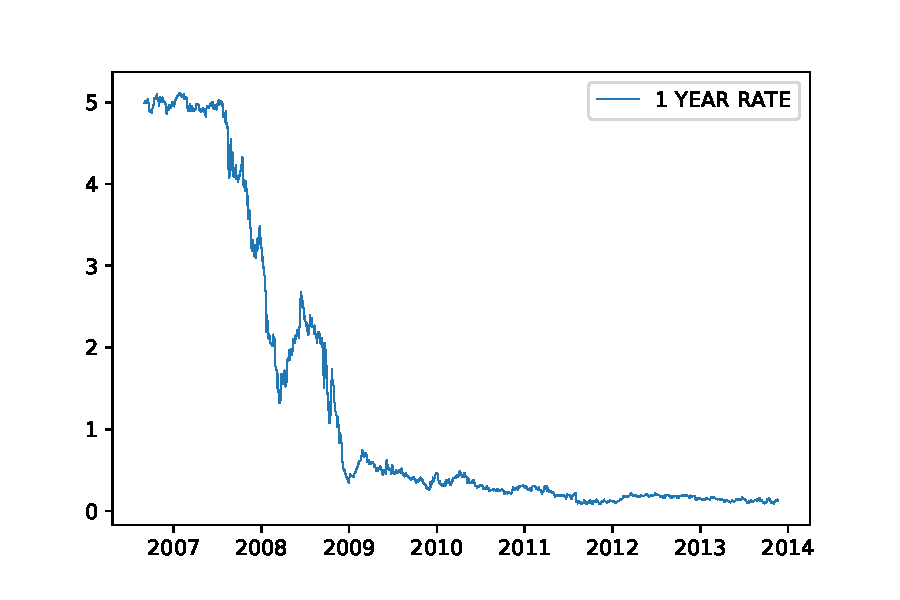
\includegraphics[width=\textwidth]{Figures/1yr.pdf}
    \end{subfigure}
    \begin{subfigure}[b]{0.32\textwidth}
    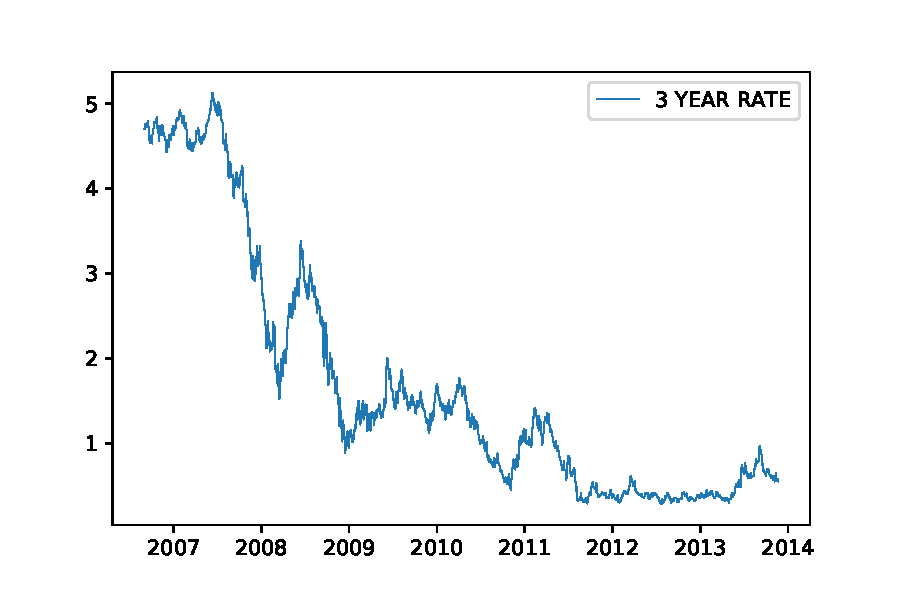
\includegraphics[width=\textwidth]{Figures/3yr.pdf}
    \end{subfigure}
    \begin{subfigure}[b]{0.32\textwidth}
    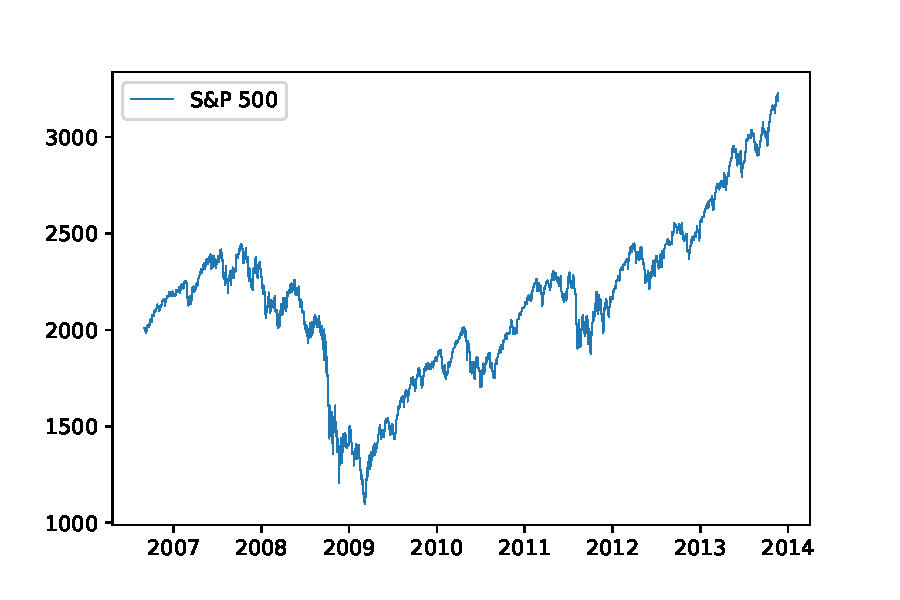
\includegraphics[width=\textwidth]{Figures/sp.pdf}
    \end{subfigure}
    \caption{Development of time series over time. 1 year rate (left), 3 year rate (middle) and S\&P 500 (right).}
    \label{fig:orig_ts}
\end{figure}

The daily percentage change is calculated to get stationary time series with mean zero. 

\begin{figure}[H]
    \centering
    \begin{subfigure}[b]{0.32\textwidth}
    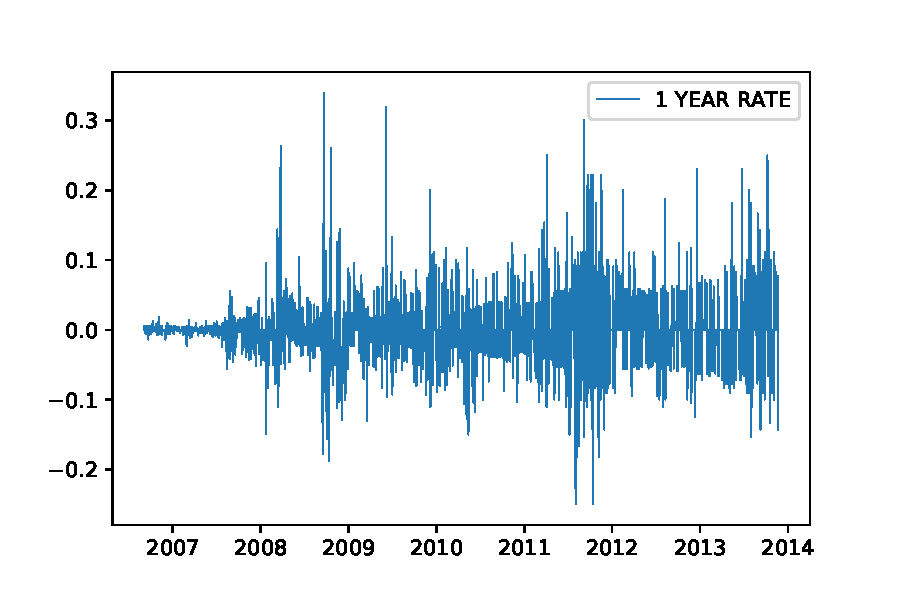
\includegraphics[width=\textwidth]{Figures/1yr_pct.pdf}
    \end{subfigure}
    \begin{subfigure}[b]{0.32\textwidth}
    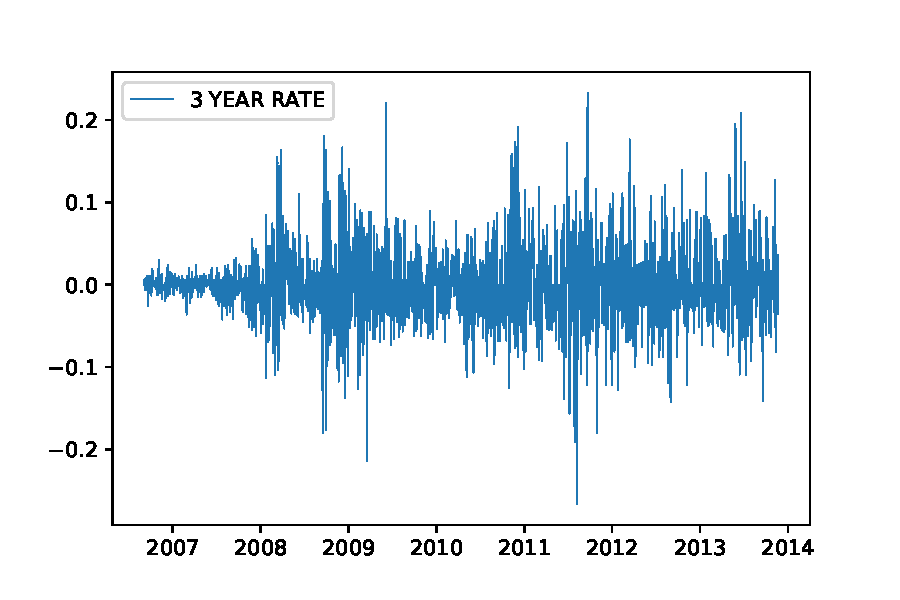
\includegraphics[width=\textwidth]{Figures/3yr_pct.pdf}
    \end{subfigure}
    \begin{subfigure}[b]{0.32\textwidth}
    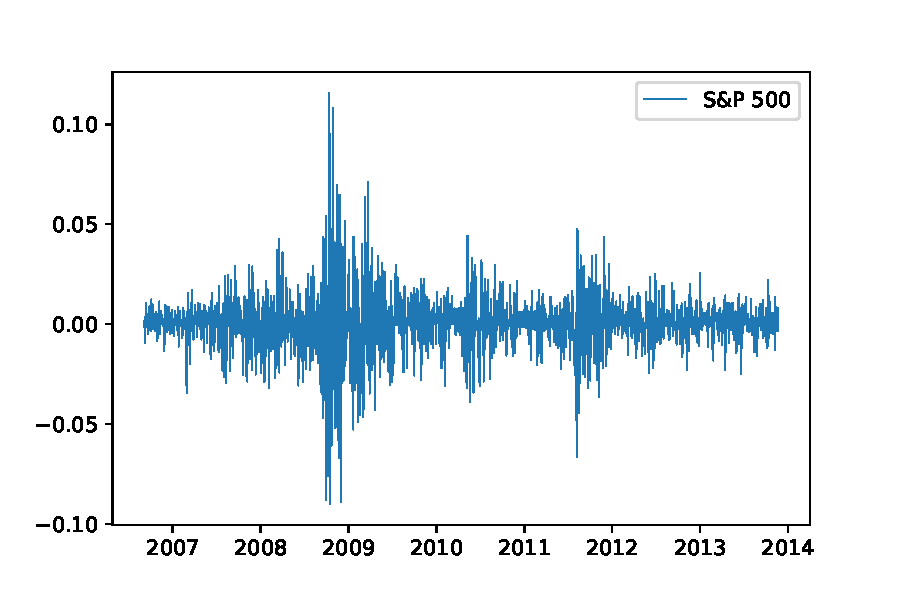
\includegraphics[width=\textwidth]{Figures/sp_pct.pdf}
    \end{subfigure}
    \caption{Daily percentage change. 1 year rate (left), 3 year rate (middle) and S\&P 500 (right).}
    \label{fig:pct_ts}
\end{figure}

To calculate ARMA predictions, I fitted a model to the available information at time $t$. A prediction is then made for time $t+1$. Since the financial news headlines are the limiting dataset in terms of dates, earlier data can be used for the time series forecasting. The time series are included from 2006-09-01 in order to make a proper prediction for the first sample in the news dataset at 2006-10-20. 

After constructing models and forecasting the time series, the forecasts are compared to the actual percentage changes. This is used to create labels for the classification task. If the ARMA prediction is higher than the actual outcome, the label is 0. Otherwise, it is 1. 
The binary accuracy -- the accuracy of the index going up or down -- of the ARMA predictions can also be used as a baseline for comparison with other models.\marginpar{Please try to use the active voice} 

I used the Python package \emph{statsmodels} to fit ARMA models and make predictions. Traditional time series analysis is not the main concern of this project. Therefore, the parameter estimation is rather crude. The AIC is calculated for a few different values of $p$ and $q$, which suggests an ARMA(1,1) process is adequate. 

\section{Text Vectorization}
Some text vectorization techniques are jointly trained with the classification model, and thus not possible to isolate from the model. Others can be trained both jointly and used as a pre-processing layer for another model. This project uses three vectorization techniques. In all of the techniques except for Sentence-BERT, the news titles for one day are concatenated in one document representing the news of this day. 

The news dataset contains 27,617 unique words when converted to lower case. 

\subsection{TF-IDF}
Term Frequency--Inverse Document Frequency (TF-IDF) is purely a pre-processing technique which outputs large dimensional vectors of the same length as the vocabulary size. This can then be fed into any model. As stated in the previous chapter, this technique does not preserve the order of words, which does not make it suitable to use as input to a recurrent network. We used a tokenizer from the scikit-learn library to transform the texts into TF-IDF vectors. 

Even though TF-IDF deals with frequency of words, there is still a computational benefit of having a restricted vocabulary, since this is equal to the input dimension. An appropriate vocabulary size is found by evaluating the validation accuracy for different sizes using logistic regression. This is because logistic regression is optimized quickly and can give an indication of when important information for classifying is lost. For the IMDb dataset, this was found to be 10,000 words. 

\subsection{GloVe}

For the word embeddings, I used the GloVe pre-trained word vectors. The vectors have been trained on a dump of Wikipedia from 2014 containing 1.6 billion tokens and the English Gigaword fifth edition dataset, containing 4.3 billion tokens \citep{pennington2014glove}. 400,000 uncased words with an embedding size of 300 dimensions are represented in the GloVe dictionary I used. Of the 22,415 words in the news data, 22,107 were available as pre-trained GloVe embeddings. 

The tokenization for the GloVe models first converted all words to lower case and reformed some words such as \textit{won't} and \textit{can't} to \textit{will not} and \textit{can not}. This allows for more words to be initialized with pre-trained embeddings since contracted words are handled differently by different tokenizers. The tokenization is done using the tokenizer from Keras.  

For the non-sequential models, the data is converted from $w \times d$ dimensions to $1 \times d$, where $w$ is the number of words in the concatenated news titles for one day and $d$ is the embedding dimensions, here 300. This is done by taking the element-wise average over all $d$ dimensions. In the models using the embeddings as non-trainable pre-processing, this is simply done before the data is fed into the model. In the models where the training of the embeddings are continued, a custom layer in Keras computes the element-wise average after the embedding layer, where the data has been inputted as token indices and the pre-trained embeddings are set in the embedding layer.

For sequential models, the order of words in the titles is kept intact. The number of words in the news titles for one day is shown in Figure~\ref{fig:num_words}. In order for each text sample to have the same size, a maximum sentence length is set. Longer sequences are cut of, shorter sequences are padded with zeros. The maximum sequence length is set to 800 for the news data, which well covers the majority of the samples. 

\begin{figure}[H]
\centering
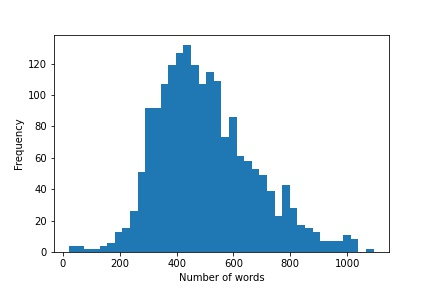
\includegraphics[width=0.8\textwidth]{Figures/wordcount.jpg}
\caption{Histogram of the number of words in the concatenated news titles for one day. }
\label{fig:num_words}
\end{figure}

\subsection{Sentence-BERT}

\citeauthor{reimers2019sentence}, the authors of Sentence-BERT,  have made models publicly available on Github, see Appendix \ref{appendix:A}. The package is called \emph{sentence-transformers}. A pre-trained model is used to embed sentences into vectors of length 768. In order to represent a full document or several news headlines, each sentence is embedded independently. The elementwise average is taken to represent the collection of sentences. These features can then be used as input to classification models. 

\subsection{BERT}

The tokenization for the BERT model is more complex than previously described models. As described in Section \ref{sec:bert_theory}, each input to BERT is made up of three vectors for every token -- \emph{token id, segment id} and \emph{mask}. The main part of this is implemented in a tokenizer supplied by \citet{devlin2018bert} on Github, see Appendix \ref{appendix:A}. Some processing is done after the tokenization, such as adding \textsc{[CLS]} and \textsc{[SEP]} tokens for the start and end of sequences. 

The maximum sequence length for BERT is 512, which implies 65 \% of the daily news headlines can not be fully represented. The first 512 tokens of these daily headlines are used in these cases. Shorter sequences are padded with zeros.  

\section{Models}

This section explains the models used in the experiments and how they are implemented.  Firstly, general feed forward-style models are described, followed by recurrent models, and lastly the transformer model BERT.  

\paragraph{Random Classifier.}
For an imbalanced rather small dataset, a random classifier can provide a basic understanding of what performance to beat to ensure some predictive power in a model. The random classifier can be trained on the training set, or just randomly predict on the test set. I have used two random classifiers which make some use of the training set. 

Two approaches were used -- \emph{stratified} and \emph{most frequent}. The stratified method respects the distribution of labels in the training data and randomly predicts on the test data with the same distribution. The most frequent-method simply predicts the most frequent label in the training data on all the test samples.

The random classifiers used in this project only relies on the target variables, so it is not interesting to classify it as sequential or not.  

\subsection{Tree-based \& Feed Forward Models}

These models are only used with non-sequential data as input, i.e. TF-IDF, average GloVe embeddings and Sentence-BERT. These vectorizations typically have dimensions 5,000--20,000 (TF-IDF), 300 (GloVe) and 768 (Sentence-BERT). 


\paragraph{Logistic Regression.}
We used logistic regression both as a traditional benchmark and a more novel model in combination with GloVe and BERT embeddings. We used the logistic regression model from the python library scikit-learn  for the implementation.

\paragraph{Support Vector Machine.}
We used a support vector machine (SVM) with similar motivation as for the logistic regression -- it serves as a well known benchmark model and is rather simple to implement and optimize.  We used a support vector machine for binary classification from the scikit-learn library. 

\paragraph{Feed-forward Network.}
A densely connected feed-forward network is evaluated with varying number of hidden layers, nodes and dropout rate. The loss function is binary cross entropy. 

The input to the model is either sequential data into an embedding layer (see Figure~\ref{fig:emb_ff}) -- if the embeddings are continuously trained -- or as pre-processed data with static embeddings. For the latter case, this is just a regular multilayer perceptron with rectified linear unit activation function and dropout regularization. The output layer is a single node with a sigmoid activation function.

The model taking sequential inputs has an embedded layer as the first layer. The weights in this layers are set to the pre-trained GloVe embeddings, and are then jointly trained with the other parameters in the model. A maximum sequence length is specified and an average is taken element-wise over all the 300 embedding dimensions. The average is taken where the sum of the absolute value of the embedding vector is non-zero, i.e. the positions in the sequence vector that actually contain a word.

\begin{figure}[t]
    \centering
    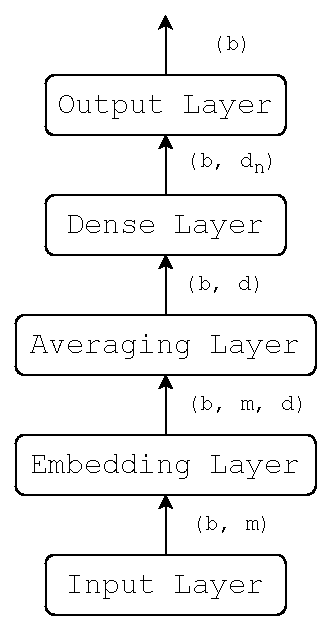
\includegraphics[width=0.3\textwidth]{Figures/figs-ff_emb.pdf}
    \caption{Schematic overview of the used feed-forward network with embedded inputs. $b$ is the batch size, $m$ is the maximum sequence length, $d$ is the embedding dimension and $d_n$ is the number of nodes in the dense layer.}
\label{fig:emb_ff}
\end{figure}

This tensor is then passed into a regular multi layer perceptron as described previously.

The feed-forward network is implemented using the Keras library. 

\subsection{Recurrent Models}

The sequential models all allow further training of embedding parameters, since the first input layer is a regular embedding layer. The input dimensions are $w \times d$, where $w$ is the maximum sequence length and $d$ is the dimension of the embedding. 

\paragraph{Bidirectional LSTM.}
The bidirectional LSTM has the same input structure as the feed-forward network, but rather than an averaging layer over all dimensions, an LSTM layer is applied. This preserves the sequential structure of the inputs and enables the model to take the order of words into account. 

The LSTM layer is wrapped in a bidirectional layer, which implies the input sequences are processed both from left-to-right and from right-to-left. Since this configuration takes a lot of time to train, hyper parameters optimization is performed by manually testing a few parameters.  

\begin{figure}[t]
    \centering
    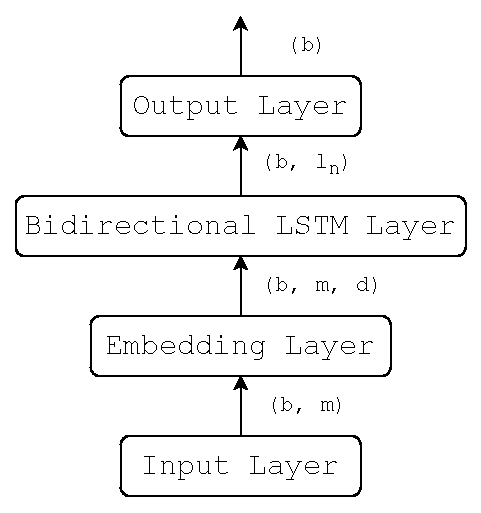
\includegraphics[width=0.4\textwidth]{Figures/figs-bidir-lstm.pdf}
    \caption{Schematic overview of a bidirectional LSTM network with sequential input data. $b$ is the batch size, $m$ is the maximum sequence length, $d$ is the embedding dimension and $l_n$ is the number of nodes in the LSTM-layer.}
\end{figure}


\subsection{Transformer Models}

One transformer model has been implemented, tuned with two different final layers. A pre-trained BERT-base model from TensorFlow hub is used and implemented as a Keras layer. The two final layers of the BERT base model are fine tuned. One model simply adds a sigmoid output node to the BERT-base model. The other model appends a hidden layer with 256 nodes and dropout regularization. 
The training is done with hyperparameters recommended by \citeauthor{devlin2018bert}, a batch size of 16 and an Adam optimizer with learning rate 2e-5. 
The benchmarking on the IMDb dataset is trained for 4 epochs. The financial dataset is significantly smaller (1,846 samples vs 20,000 samples) and is thus trained using an early stopping callback conditioned on validation accuracy.  

\begin{figure}[t]
    \centering
    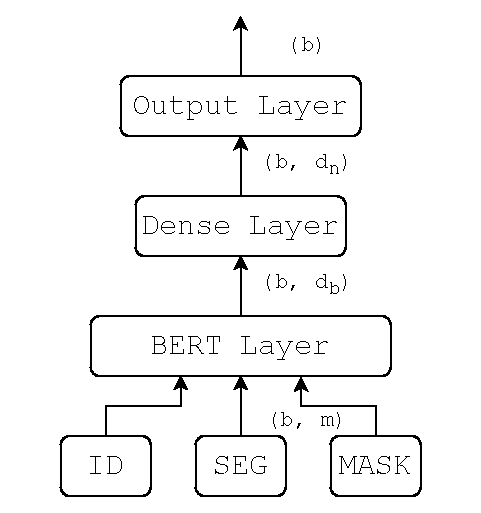
\includegraphics[width=0.4\textwidth]{Figures/figs-bert-ff.pdf}
    \caption{Schematic overview over the architecture of the BERT model. $b$ is the batch size, $m$ is the maximum sequence length, $d_b$ is the BERT embedding dimension and $d_n$ is the number of nodes in the dense layer.}
\end{figure}


\section{Hyperparameter Optimization}

The selection of hyperparameters was carried out using either a grid search or a random search over a selected range of parameters. Grid search was used for random forest and random search was used for other models where hyperparameter optimization was made. The search was done with either 10 or 3 fold cross-validation depending on the computational feasability. More demanding models like bidirectional LSTM and BERT were fitted by manual tuning of hyperparameters, i.e. using values that seem reasonable. 

The neural network-style models were trained using an early-stopping callback. This implies that the model is trained until the validation accuracy has not improved for a number of epochs. The final model is then chosen as the model with the highest validation accuracy. 

The tested ranges and concluded sets of parameters for a selection of models are listed in Appendix \ref{appendix:B}.

\section{Implementation Notes}

All optimizations are carried out on in a Jupyter notebook environment using python 3.7.4 and TensorFlow 1.15. Python is run on a local computer with 16 GB RAM and an Intel i7-10510U CPU, 1.80 GHz. 